\chapter*{Acerca del Autor}

% ============================================
% PERFIL PRINCIPAL
% ============================================
\begin{tcolorbox}[colback=gray!5!white, colframe=blue!75!black]
	\begin{minipage}[c]{0.35\linewidth}
		\centering
		% Foto del autor — colocar imagen en Figures/carnet.png
		\setlength{\fboxsep}{0pt}
		\fbox{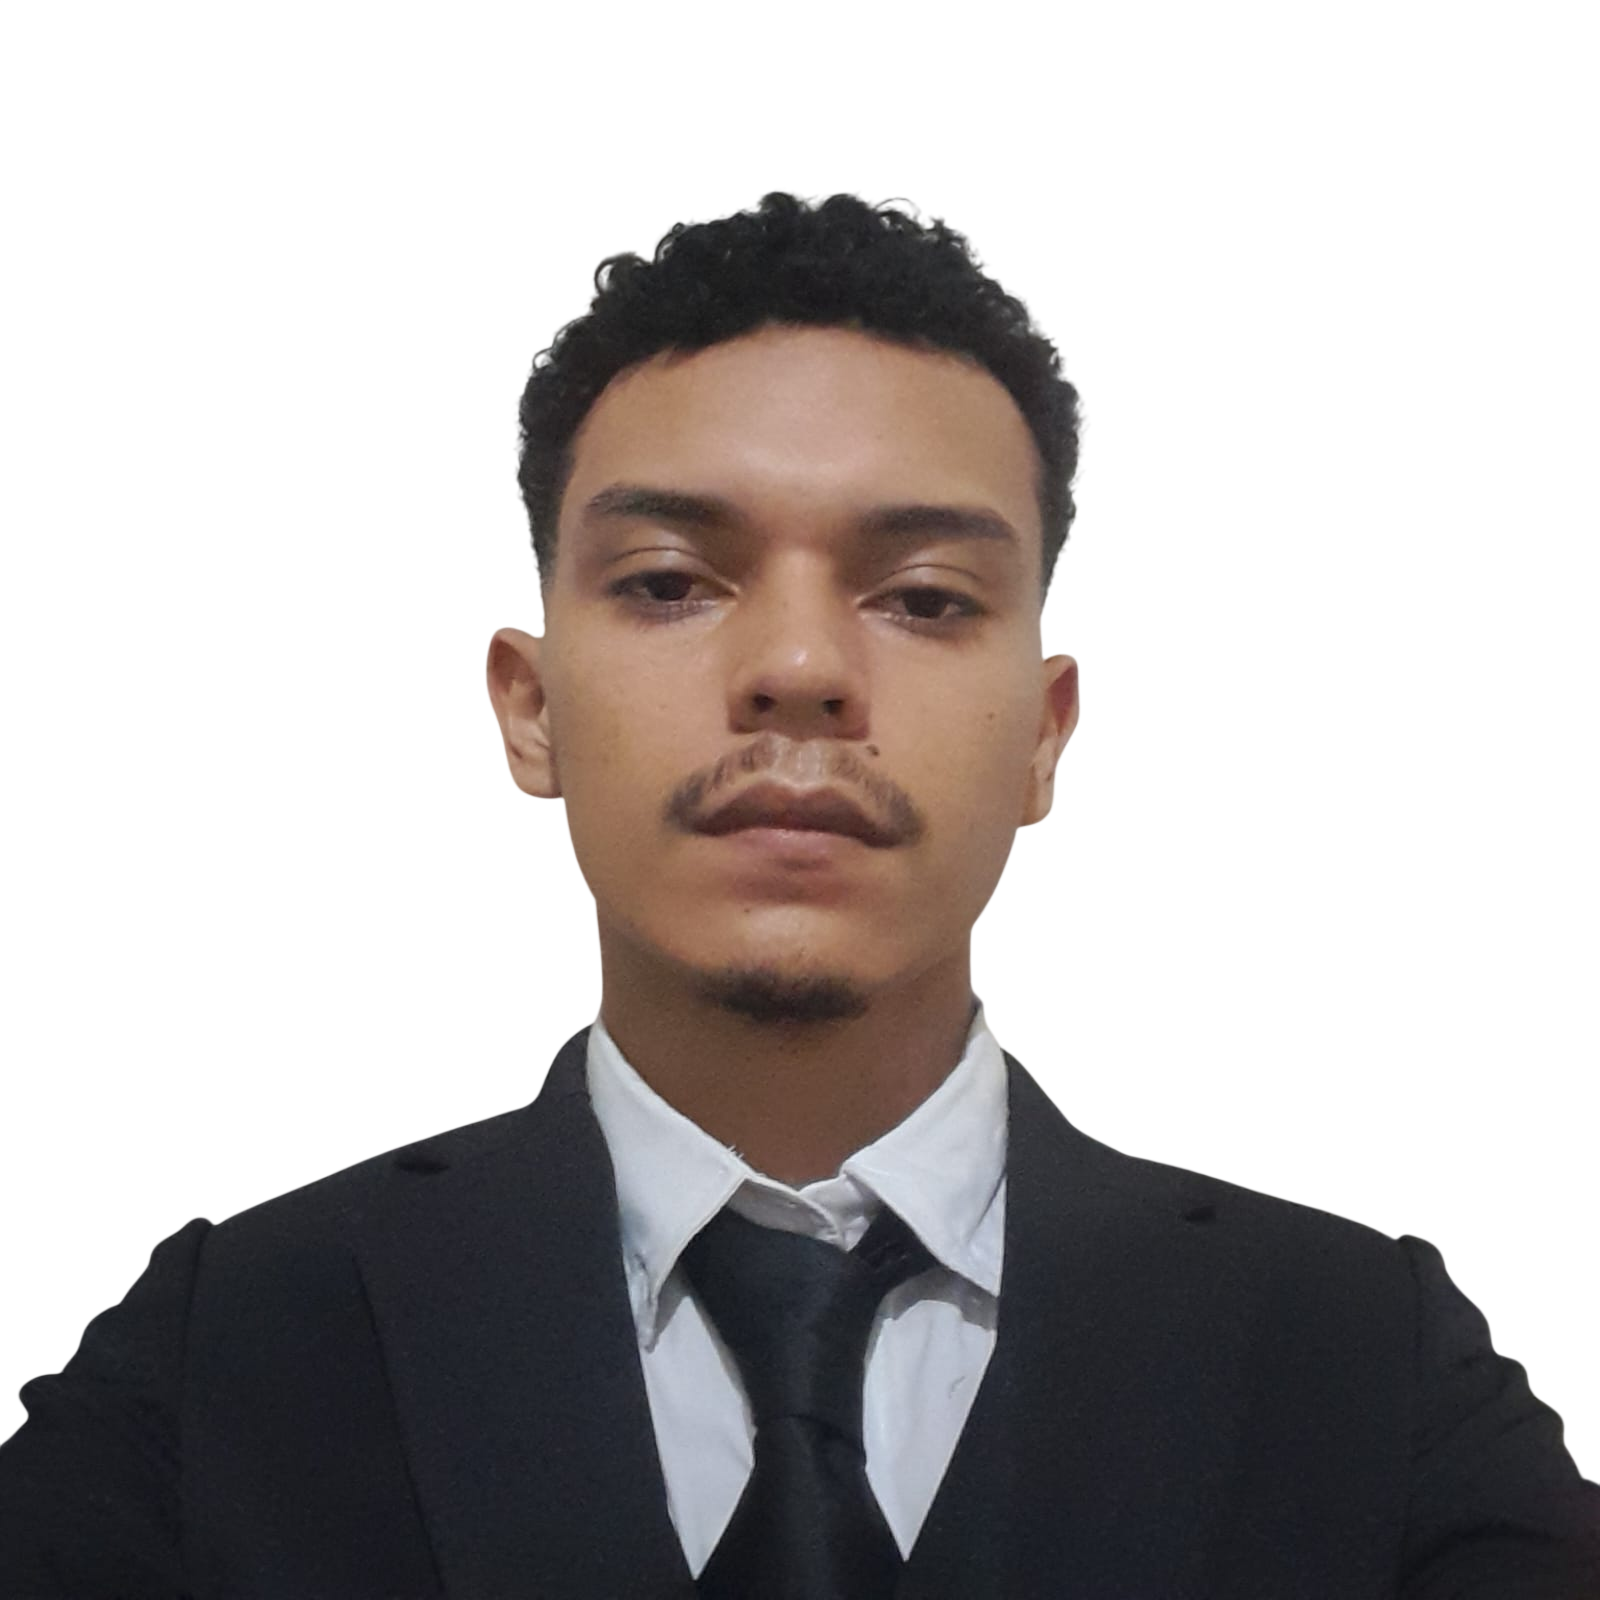
\includegraphics[width=\linewidth]{Figures/carnet.png}}
	\end{minipage}
	\hfill
	\begin{minipage}[c]{0.6\linewidth}
		\textbf{\large José Manuel Romero Martínez} \\[0.2cm]
		\textit{Estudiante de Ingeniería en Sistemas} \\
		Universidad Nacional Autónoma de Honduras \\
		Campus Comayagua

		\vspace{0.4cm}

		\begin{tabular}{@{}ll}
			\faOrcid\ ORCID: & \href{https://orcid.org/0009-0001-0780-7160}{0009-0001-0780-7160} \\[0.1cm]
			\faGraduationCap\ Google Scholar: & \href{https://scholar.google.com/citations?hl=es&user=uER9hnEAAAAJ}{José Manuel Romero Martínez} \\[0.1cm]
			\faLinkedin\ LinkedIn: & \href{https://www.linkedin.com/in/jos\%C3\%A9romero/}{/in/joséromero} \\[0.1cm]
			\faGithub\ GitHub: & \href{https://github.com/Josemaromero46}{@Josemaromero46} \\[0.1cm]
			\faEnvelope\ Email: & \href{mailto:romeromanuel@unah.hn}{romeromanuel@unah.hn}
		\end{tabular}
	\end{minipage}
\end{tcolorbox}

\vspace{0.4cm}

% ============================================
% RESEÑA BIOGRÁFICA
% ============================================
\noindent

Estudiante de Ingeniería en Sistemas en la Universidad Nacional Autónoma de Honduras, Campus
Comayagua. Su formación combina desarrollo de software, inteligencia artificial aplicada y
desarrollo móvil multiplataforma.

Ha participado en proyectos académicos y freelance en desarrollo móvil, \textit{backend} y
\textit{frontend}, trabajando con interfaces responsivas, componentes reutilizables y consumo
de \textit{APIs} REST. Entre sus proyectos destaca el desarrollo de una aplicación de torneos
de fútbol multiplataforma con Flutter y PocketBase. Cuenta además con experiencia en
configuración de redes y laboratorios universitarios.

\vspace{0.4cm}

% ============================================
% COMPETENCIAS TÉCNICAS
% ============================================
\noindent\textbf{Competencias Técnicas:}

\vspace{0.2cm}

\noindent
\textbf{Lenguajes:} C\#, C++, Java, Python, JavaScript, TypeScript, SQL, Prolog, \LaTeX{} \\
\textbf{Frontend:} HTML5, CSS3, Tailwind CSS, React, Next.js \\
\textbf{Frameworks:} Flutter, Node.js, Express.js, Firebase, Bootstrap, Spring \\
\textbf{Bases de datos:} MySQL, SQL Server, Oracle DB \\
\textbf{Herramientas:} Git, GitHub, Android Studio, VS Code, Figma, Canva \\
\textbf{Idiomas:} Español (nativo), Inglés (B1)

\MediaOptionLogic
